
\subsubsection{MHUI main}

\begin{figure}[ht]
\centering
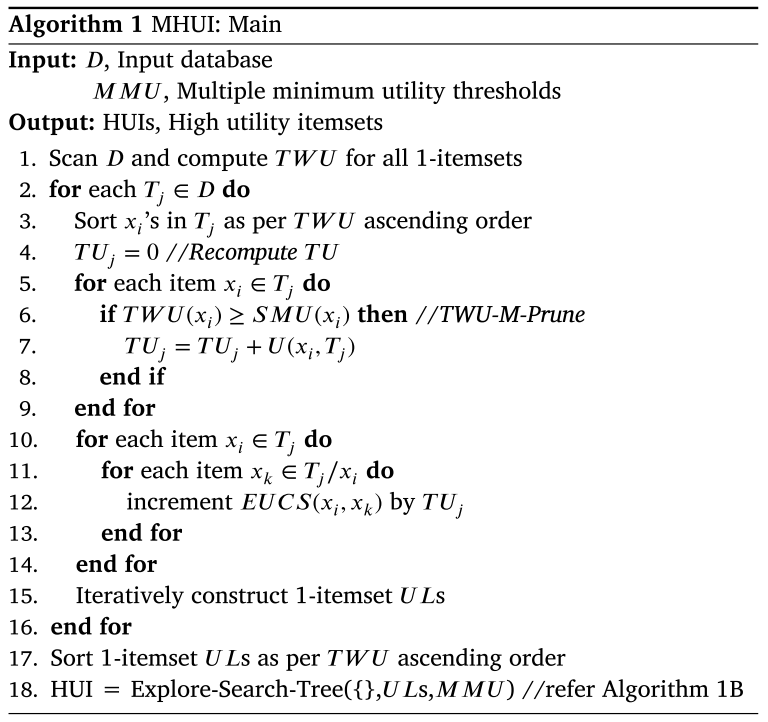
\includegraphics[width=0.9\textwidth]{image/algo/algo1.PNG}
\caption{\label{fig:algo1} MHUI main}
\end{figure}

\paragraph{Dữ liệu đầu vào} Cơ sở dữ liệu D, ngưỡng giá trị tiện ích tối thiểu cho từng món hàng.  
\paragraph{Dữ liệu đầu ra} HUIs, tập các itemset có giá trị tiện ích cao.\\



Hình \ref{fig:algo1} là hàm bắt đầu chương trình. Chương trình sẽ tính các TWU (tạo ra bảng như hình\ref{fig:table4}), dòng 1 trong thuật toán, đây là lần duyệt cơ sở dữ liệu đầu tiên. Sau đó, chương trình duyệt qua cơ sở dữ liệu lần 2, ở mỗi giao dịch $T_j$ chương trình sẽ làm những việc sau đây trong mỗi vòng lập qua 1 giao dịch.

\begin{itemize}
  \item Sắp xếp các món hàng trong giao dịch theo thứ tự TWU (dòng 3). 
  \item Tính lại TU cho mỗi giao dịch sau khi áp dụng phương pháp tỉa cây TWU-M-Prune. (dòng 6, 7)
  \item Tính EUCS dựa vào TU sau khi tỉa cây TWU-M-Prune (dòng 12)
  \item Từ từ xây dựng 1-itemset utility list (gọi tắt ULs) như hình \ref{fig:1itemset} (dòng 15) 
\end{itemize}

Sau khi kết thức vòng lập, sắp xếp ULs theo thứ tự TWU (dòng 17), gọi hàm Explore-Search-Tree (dòng 18). 

\subsubsection{Hàm duyệt cây: Explore-Search-Tree }

\begin{figure}[ht]
\centering
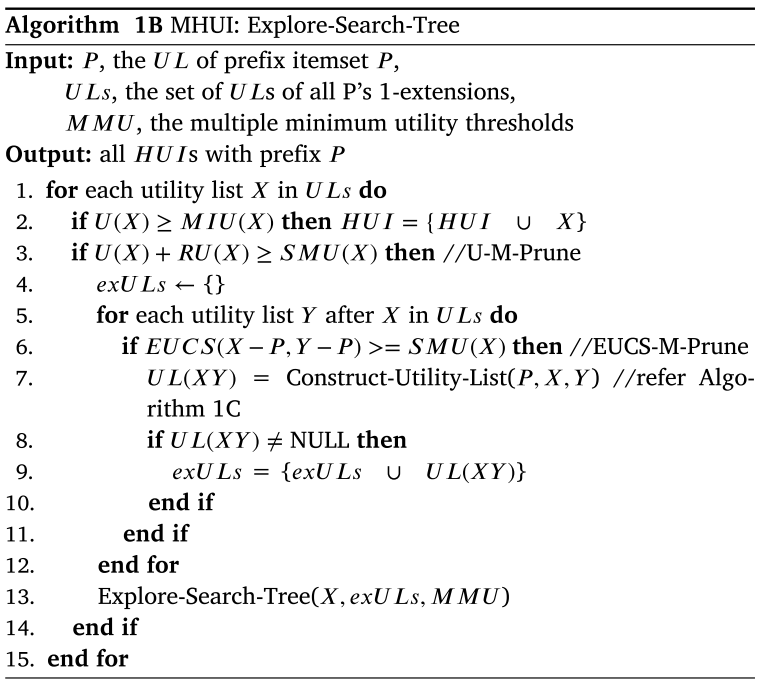
\includegraphics[width=0.9\textwidth]{image/algo/algo2.PNG}
\caption{\label{fig:algo2} MHUI Explore Search Tree}
\end{figure}

\paragraph{Dữ liệu đầu vào} Một itemset gọi là P, tập hợp có thứ tự các itemset ULs, ngưỡng giá trị tiện ích tối thiểu cho từng món hàng.

\paragraph{Dữ liệu đầu ra} HUIs với tiền tố P \\

Hàm duyệt cây (hình \ref{fig:algo2}) sẽ kiểm tra cái nút tại đó xem nó có là HUI không (có $U(X) \geq MIU(X)$ ) đê gắn nút vào danh sách HUI trả về cuối cùng. Hàm duyệt cây theo Depth First Search, nghĩa là nó sẽ duyệt một nút sâu nhất có thể, sau đó mới chuyển qua nút tiếp theo. Một nút chỉ được duyệt khi nó thỏa U-M-Prune. 

Quá trình duyệt cây sẽ lập qua mỗi X trong tập ULs. Nếu X thóa U-M-Prune, rồi vòng lập con lập qua mỗi Y theo sau X trong ULs (ULs đã xếp theo thứ tự TWU), và thực hiện 2 việc sau 

\begin{itemize}
  \item kiểm tra P, X, Y thỏa EUCS-M-Prune (dòng 6), bỏ qua vòng lập này nếu không thỏa   
  \item xây dựng danh sách UL (dòng 7). Sẽ gọi hàm \ref{fig:algo3} để tạo ra UL. 
  \item gộp vào dãy exULs (dòng 8) 
\end{itemize}
 
Sau mỗi vòng lập ngoài (vòng lập của X) thuật toán gọi đệ quy gọi đệ quy Explore-Search-Tree(X, exULs) để duyệt cây theo depth first search. 

\subsubsection{Xây dựng dãy tiện ích: Construct-Utility-List }

\paragraph{Dữ liệu đầu vào} UL itemset P, itemset Px, và itemset Py 

\paragraph{Dữ liệu đầu ra} UL của itemset Pxy \\

\begin{figure}[ht]
\centering
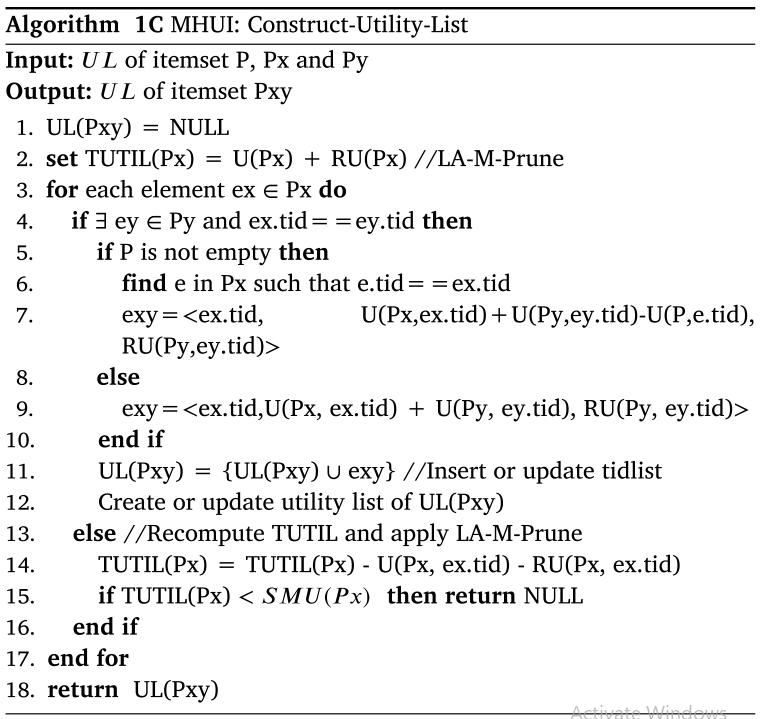
\includegraphics[width=0.9\textwidth]{image/algo/algo3.PNG}
\caption{\label{fig:algo3} MHUI Construct Utility List}
\end{figure}

Thuật toán tạo dãy Utility như hình \ref{fig:algo3} sẽ tạo ra UL mới từ 2 bằng cách ghép 2 UL Px và Py. Cả 2 UL Px và Py đều có chung tiền tố P. Thuật toán sẽ áp dụng LA-M-Prune và trả về NULL (rỗng) khi Px và Py không thỏa điều kiện. 

Kết quả trả về sẽ như một cột như hình \ref{fig:1itemset}, bao gồm itemset và mỗi dãy các bảng ghi có dạng <tid, U, RU>. 
